\documentclass[acmsmall,screen]{acmart}

\def\BibTeX{{\rm B\kern-.05em{\sc i\kern-.025em b}\kern-.08em
    T\kern-.1667em\lower.7ex\hbox{E}\kern-.125emX}}
\usepackage{paralist}
\usepackage{amsmath,amsfonts}
\usepackage{array}
% \usepackage[caption=false,font=normalsize,labelfont=sf,textfont=sf]{subfig}
\usepackage{textcomp}
\usepackage{stfloats}
\usepackage{url}
\usepackage{verbatim}
\usepackage{graphicx}
% \usepackage{cite}
\usepackage[ruled,vlined,linesnumbered]{algorithm2e}
\usepackage{algpseudocode}
\usepackage{xcolor}
\usepackage{multirow}
\usepackage{amsfonts}
\usepackage{xspace}
\usepackage{colortbl}
\usepackage{makecell}
\usepackage{microtype}
\usepackage{enumitem}
\usepackage{pifont}
\usepackage{booktabs}
\usepackage[switch]{lineno}
\usepackage{tcolorbox}
\newtcolorbox{ansbox}{colframe = gray!75!black}
\usepackage{subcaption}



\newcommand{\tool}{\textit{MoDitector}\xspace}
\newcommand{\oracle}{\textit{Module-Specific Oracle}\xspace}
\newcommand{\select}{\textit{Adaptive Seed Generation}\xspace}
\newcommand{\feedback}{\textit{Module-Specific Feedback}\xspace}


\newcommand{\mccs}{$\mathcal{M}\text{ICS}$\xspace}
% \newcommand{\Fmccs}{$$\mathbf{F}_{\mathcal{M}^{k}}$$\relax\xspace}
\newcommand{\abb}{\textit{MoDitector}\xspace}
\newcommand{\colorit}{\cellcolor{gray!25}}

\newcommand{\todo}[1]{\textbf{\textcolor{red}{TODO: #1}}}




\title{\tool: Module-Directed Testing for Autonomous Driving Systems}

% \author{Ben Trovato}
% \authornote{Both authors contributed equally to this research.}
% \email{trovato@corporation.com}
% \orcid{1234-5678-9012}
% \author{G.K.M. Tobin}
% \authornotemark[1]
% \email{webmaster@marysville-ohio.com}
% \affiliation{%
%   \institution{Institute for Clarity in Documentation}
%   \city{Dublin}
%   \state{Ohio}
%   \country{USA}
% }

\author{Renzhi Wang}
\authornote{Both authors contributed equally to this research.}
\authornote{This work was done during the author's visit to Singapore Management University}
\orcid{0000-0002-1219-0732}
\affiliation{%
  \institution{University of Alberta}
  \city{Edmonton}
  \state{Alberta}
  \country{Canada}}
\email{renzhi.wang@ualberta.ca}

\author{Mingfei Cheng}
\authornotemark[1]
\orcid{0000-0002-8982-1483}
\affiliation{%
  \institution{Singapore Management University}
  \city{Singapore}
  \country{Singapore}
}
\email{mfcheng.2022@smu.edu.sg}

\author{Xiaofei Xie}
\orcid{0000-0002-1288-6502}
\affiliation{%
 \institution{Singapore Management University}
 \city{Singapore}
 \country{Singapore}}
\email{xfxie@smu.edu.sg}

\author{Yuan Zhou}
\authornote{Corresponding author.}
\orcid{0000-0002-1583-7570}
\affiliation{%
  \institution{Zhejiang Sci-Tech University}
  \city{Hangzhou}
  \state{Zhejiang}
  \country{China}}
\email{zhouyuan1130@163.com}

\author{Lei Ma}
\orcid{0000-0002-8621-2420}
\affiliation{%
  \institution{The University of Tokyo \& University of Alberta}
  \city{Tykyo}
  \country{Japan}}
\email{ma.lei@acm.org}

\date{\today}

\begin{document}

\begin{abstract}
Testing Autonomous Driving Systems (ADS) is crucial for ensuring their safety, reliability, and performance. Despite numerous testing methods available that can generate diverse and challenging scenarios to uncover potential vulnerabilities, these methods often treat ADS as a black-box, primarily focusing on identifying system failures like collisions or near-misses without pinpointing the specific modules responsible for these failures. Understanding the root causes of failures is essential for effective debugging and subsequent system repair. We observed that existing methods also fall short in generating diverse failures that adequately test the distinct modules of an ADS, such as perception, prediction, planning and control.

To bridge this gap, we introduce \tool, the first root-cause-aware testing method for ADS. Unlike previous approaches, \tool not only generates scenarios leading to collisions but also showing which specific module triggered the failure. This method targets specific modules, creating test scenarios that highlight the weaknesses of these given modules. Specifically, our approach involves designing module-specific oracles to ascertain module failures and employs a module-directed testing strategy that includes module-specific feedback, adaptive seed selection, and mutation. This strategy guides the generation of tests that effectively provoke module-specific failures. We evaluated \tool across four critical ADS modules and four testing scenarios. The results demonstrate that our method can effectively and efficiently generate scenarios where errors in targeted modules are responsible for ADS failures. It generates 216.7 expected scenarios in total, while the best-performing baseline detects only 79.0 scenarios. 
Our approach represents a significant innovation in ADS testing by focusing on identifying and rectifying module-specific errors within the system, moving beyond conventional black-box failure detection.
\end{abstract}

\keywords{Module-Specific Failure, Autonomous Driving System, Testing}
\maketitle


Stochastic systems have been used extensively in several areas including  verification~\cite{FKNP11}, learning theory~\cite{AJKS21}, epidemic processes~\cite{Lef81} to name a few. Several real-world systems however do not work with a centralised control. Therefore, modelling using stochastic systems with multiple agents makes for more faithful abstractions of such systems without a centralised control. Some examples of fields in which multi-agents stochastic modelling include cyber physical systems~\cite{SEC16}, distributed and probabilistic computer programs~\cite{dAHJ01}, probabilistic planning~\cite{TKI10}. In such cases, the problem of reasoning about multiple agents with several, often times orthogonal objectives, becomes important. % However, for situations that are modelled as graph games, Nash equilibria come with its own down-sides and therefore several notions of equilibria have emerged in turn-based games on graphs to circumvent the problems posed by the natural definitions of Nash equilibira, like subgame-perfect equilibira, Stackleberg-equilibria. 
For multi-agent systems modelled with stochasticity on the underlying arena, a fundamental question to ask is the existence or finding of an equilibrium.
The most popular equilibria in literature are Nash equilibria~\cite{Nas50}. However, those come with their own downsides. The computational complexity for studying Nash equilibria over multi-agent systems is prohibitively expensive, and even undecidable in the general case, where systems have $10$ or more players~\cite{UW11}. 
Further, even if Nash equilibria could be computed efficiently, they do not faithfully model the agents in real world settings
%as each agent might perceive risk differently. With randomness arising from both the strategies of other agents, as well as the underlying model of the system, this might mean that risk-averse or risk-loving agents might have an incentive to deviate since their perceived values of outcome is different from expected value of the game.
since they do not consider their tolerance or averseness to risk.

Let us consider a $1$-player game where a protagonist is proposed two options: (a) earning \$1; (b) playing a lottery in which, with probability $\frac{1}{40}$, she gets \$40, and with probability $\frac{39}{40}$, she does not earn anything.
Classically, rational strategies would be maximising the expected payoff. From this perspective, both options yield an expected payoff of \$1, making them equivalent.
This approach is particularly justified when the game represents a scenario that can be repeated many times: the law of large numbers ensures that, in the long run, the average payoff will converge to the expected payoff. However, when the game is played only once, the protagonist may prioritise immediate needs. If she urgently requires \$1, the guaranteed option (a) becomes preferable.

Conversely, if she is a risk-taker or finds herself in a situation where only the \$40 can make a significant difference, she may prefer the high-risk option (b).
Although this choice might appear irrational, it mirrors the behaviour of millions of people who participate everyday in games with a negative expected payoff, driven by the allure of a potentially life-changing win, and generating an annual turnover of USD 536 billions~\cite{GamblingNewspaper23} for the gambling industry.
That industry, on the other hand, operates on a large scale where expected payoff becomes the key metric. 
This contrast underscores the importance of alternative measures to expected payoff that account for each agent's risk tolerance.%, offering a more nuanced understanding of decision-making in uncertain scenarios.

%We thus have an example of a two-player interaction, with apparently zero-sum payoffs, but where both players express a preference for the same option, because the context gives them a different tolerance to risk: this paradox underscores the importance of alternative measures to expected payoff that account for an agent's risk tolerance, offering a more nuanced understanding of decision-making in uncertain scenarios.
% This contrast underscores the relevance of generalising the notion of Nash equilibria: in a multi-agent system, the agents may have diverging perception of which risks can be taken.
% It makes sense, then, to study \emph{risk-sensitive equilibria}, in which players do not necessarily maximise their expected payoff, but their perception of what their payoff will be according to different risk measures.\leon{I'm actually not satisfied with this, I will modify it and move it.}


% Classically, we consider that a rational strategy would consist in maximising the expected payoff: from that perspective, the two choices are equivalent.
% Such an approach is justified especially when the game models a situation that can be repeated a large number of times, in which case the law of large numbers guarantees that the average payoff converges to the expected payoff.
% But when the game models a situation that is played only once, the protagonist may consider that she really needs her euro, and that the possibility of earning 40\$ is too unlikely to be taken into account: she would then have a justifiable preference for the option (a).
% On the contrary, if she is more of a gambler, or if she finds herself in a desperate situation in which only earning those 40\$ could save her, she could go all out and express a strict preference for option (b)\footnote{Even though this case seems more irrational, it explain why millions of people play everyday games in which they know that their expected payoff is negative.
% On the other side, the companies with whom they interact repeat the experience often enough to consider expected payoff as the relevant measure --- generating a yearly turnover of 536 billions of US\$.}.
% Hence the relevance of alternatives to expected payoff, that take into account the tolerance of the agent to risk.

\subparagraph*{Risk Measures.}
A \emph{risk measure} captures the perception that a player has of what their payoff will be. In that sense, they generalise the notion of expected payoff.
Various risk measures exist in the literature, and have been used extensively in the field of economics and finance. 
Some of these risk measures include expected shortfall (ES), value at risk (VaR)~\cite{Aue18}, variance~\cite{Bra99}, entropic risk measure (ER)~\cite{FS02}. 

%However, since the introduction of the characteristic of risk measure called \emph{coherence}~\cite{ADJH99}, it was expected that a ``good'' a risk measure must be coherent. A risk measure is coherent if it is monotonic, homogeneous, translational-invariance, and sub-additive.
%This automatically weeds out several of the above risk measures listed above like  Value at Risk or variance as a risk measure. 
A lot of work has been done in considering these risk measures over MDPs which use variance (along with mean) as a risk-measure~\cite{FK89, PSB22,MT11}, ES~\cite{RRS15,KM18,Meg22} (also referred to as conditional value at risk (CVaR), average value at risk (AVaR), expected tail loss (ETL), and superquantile in literature) and ER~\cite{HM72,BR14,BCMP24}. % have also been studied. 
Studying the entropic risk measure in MDPs appears more practical compared to expected shortfall  or using variance-penalised risk-measures. This impracticability of ES and variance-penalised measure in particular is due to the intractable exponential memory~\cite{HK15} and time required to compute optimal strategies~\cite{PSB22}, even for the one agent system of Markov decision processes (MDPs). On the other hand, when the risk measure used is ER, players have optimal positional strategies in MDPs~\cite{How72}, which makes it a prime candidate for consideration in multi-agent settings.

\subparagraph*{Entropic Risk Measure.}
The entropic risk measure is computed by assigning to each agent a risk parameter, i.e., a value $\rho \in \Rb$.
%Based on this risk parameter $\rho$, this measure first computes the expectation of the exponential function of the random variable and then re-normalises this.  
The entropic risk measure of a random variable $X$ is then defined as
$\re_\rho[X] = -\frac{1}{\rho} \log_e \left( \Eb \left[ e^{-\rho X}\right] \right)$. 
%For computational reasons, instead of the Euler's constant $e$, we use different bases sometimes.
If the risk parameter $\rho$ is positive, then more weight will be given to the bad payoffs: the corresponding player can then be considered as risk-averse.
Conversely, players with a negative $\rho$ are more risk-loving.
When $\rho$ tends to $0$, the entropic risk measure converges to the classical expectation $\Eb[X]$.

The game depicted by Figure~\ref{fig:example_gamma} extends the lottery example we discussed earlier. 
Black vertices are stochastic, and the circle vertex is controlled by player $\Circle$.
A play can be seen as an infinite sequence of moves of a token along the edges of the graph, starting from $a$: from a stochastic vertex, it takes one of the outgoing edges with the probabilities indicated on those, and from a vertex controlled by the player, she chooses which edge it takes.
The payoff $40$, $0$, or $1$ is obtained when the terminal vertex $t_1$, $t_2$, or $t_3$ is reached, respectively.
If no terminal vertex is reached, then the payoff is $0$.
Taking the red edge corresponds to option (a): then, her risk entropy is always $1$, for every risk parameter $\rho$.
But if she chooses option (b), that is, if she takes the blue edge, her risk entropy is $\re_\rho[\mu_{\circ}] = -\frac{1}{\rho} \log \left( \Eb \left[ e^{-\rho \mu_{\circ}}\right] \right) = -\frac{1}{\rho} \log \left(  e^{-40\rho } + \frac{39}{40} \right)$.
Both cases are illustrated with red and blue curves in \cref{fig:example_plot}.
The curves cross at abscissa $\rho = 0$, where the entropic risk measure corresponds to the expectation. Note that other strategies are possible if \emph{randomisation} is allowed---the player could, for example, toss a coin and participate in the lottery if the outcome is heads. The perceived reward of randomising between outermost red and blue edges are illustrated in the intermediate cases with mixtures of red and blue in \cref{fig:example_plot}.

%For this example, we  replace Euler's constant $e$ with instead the constant $2$, which makes $\re_\rho[X] = -\frac{1}{\rho} \log_2 \left( \Eb \left[ 2^{-\rho X}\right] \right)$.

%Player $\Circle$ gets the payoff $11$ if she reaches the terminal vertex $t_1$, the payoff $1$ if she reaches $t_2$, the payoff $2$ if she reaches $t_3$, and the payoff $0$ if she reaches none of those terminal states (i.e., if she loops on the vertex $a$ forever).

%If the player's strategy is to choose the red edge, she gets payoff $1$ with probability $1$.
%Therefore, her risk measure is equal to $1$ for every risk parameter $\rho$.

%If her strategy is to choose the blue edge going to $c$, then she gets the payoff $11$ with probability $\frac{1}{10}$, and $1$ with probability $\frac{9}{10}$.
%Thus her risk entropy is
%$\re_\rho[\mu_{\circ}] = \frac{1}{\rho} \log_2\left(\frac{1}{3} 2^{-4\rho} + \frac{2}{3} 2^{-1\rho}\right)$.
 
\begin{figure}[h] 
			\centering
            \begin{subfigure}[t]{0.4\textwidth}
			\begin{tikzpicture}[->,>=latex,shorten >=1pt, initial text={}, scale=1, every node/.style={scale=1}]
				\node[initial left, stoch] (a) at (0, 0) {$a$};
				\node[state] (b) at (1.5, 0) {$b$};
                \node[stoch] (c) at (2.5, 1) {$c$};
                \node (t1) at (4, 2) {$t_1:~\stack{\circ}{40}$};
                \node (t2) at (4, 0) {$t_2:~\stack{\circ}{0}$};
                \node (t3) at (3, -1) {$t_3:~\stack{\circ}{1}$};
                \path (a) edge[loop above] node[above] {$\frac{1}{2}$} (a);
				\path (a) edge node[above] {$\frac{1}{2}$} (b);
                \path (b) edge[blue, thick] (c);
                \path (b) edge[red, thick] (t3);
				\path (c) edge node[above] {$\frac{1}{40}$} (t1);
				\path (c) edge node[below] {$\frac{39}{40}$} (t2);
			\end{tikzpicture}
			\caption{A stochastic MDP}
			\label{fig:example_gamma}
            \end{subfigure}
            \begin{subfigure}[t]{0.55\textwidth}
			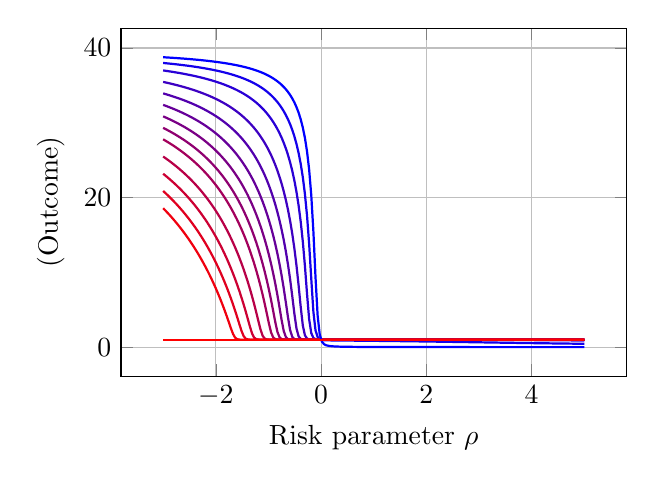
\begin{tikzpicture}
              \begin{axis}[
                xlabel={Risk parameter $\rho$},
                ylabel={$\re(\text{Outcome})$},
                domain=-3:5,
                samples=200,
                    width=8cm,
                   height=6cm,
                grid=major,
                ]
                \addplot [
                  red!8!blue,
                  thick
                ]
                {-1/x * log2((9/10)*e^(-1*x) + (1/400) * e^(-40*x) + (39/400))/log2(e)};
                \addplot [
                  red!16!blue,
                  thick
                ]
                {-1/x * log2((199/200)*e^(-1*x) + (1/8000) * e^(-40*x) + (39/8000))/log2(e)};
                \addplot [
                  red!24!blue,
                  thick
                ]
                {-1/x * log2((19999/20000)*e^(-1*x) + (1/800000) * e^(-40*x) + (39/800000))/log2(e)};
                \addplot [
                  red!32!blue,
                  thick
                ]
                {-1/x * log2((1999999/2000000)*e^(-1*x) + (1/80000000) * e^(-40*x) + (39/80000000))/log2(e)};
                \addplot [
                  red!40!blue,
                  thick
                ]
                {-1/x * log2((199999999/200000000)*e^(-1*x) + (1/8000000000) * e^(-40*x) + (39/8000000000))/log2(e)};
                \addplot [
                  red!48!blue,
                  thick
                ]
                {-1/x * log2((19999999999/20000000000)*e^(-1*x) + (1/800000000000) * e^(-40*x) + (39/800000000000))/log2(e)};
                \addplot [
                  red!56!blue,
                  thick
                ]
                {-1/x * log2((1999999999999/2000000000000)*e^(-1*x) + (1/80000000000000) * e^(-40*x) + (39/80000000000000))/log2(e)};
                \addplot [
                  red!64!blue,
                  thick
                ]
                {-1/x * log2((199999999999999/200000000000000)*e^(-1*x) + (1/8000000000000000) * e^(-40*x) + (39/8000000000000000))/log2(e)};
                \addplot [
                  red!72!blue,
                  thick
                ]
                {-1/x * log2((199999999999999999/200000000000000000)*e^(-1*x) + (1/8000000000000000000) * e^(-40*x) + (39/8000000000000000000))/log2(e)};
                \addplot [
                  red!80!blue,
                  thick
                ]
                {-1/x * log2((199999999999999999999/200000000000000000000)*e^(-1*x) + (1/8000000000000000000000) * e^(-40*x) + (39/8000000000000000000000))/log2(e)};
                \addplot [
                  red!88!blue,
                  thick
                ]
                {-1/x * log2((199999999999999999999999/200000000000000000000000)*e^(-1*x) + (1/8000000000000000000000000) * e^(-40*x) + (39/8000000000000000000000000))/log2(e)};
                \addplot [
                  red!94!blue,
                  thick
                ]
                {-1/x * log2((199999999999999999999999999/200000000000000000000000000)*e^(-1*x) + (1/8000000000000000000000000000) * e^(-40*x) + (39/8000000000000000000000000000))/log2(e)};
                \addplot [
                  blue,
                  thick
                ]
                {-1/x * log2((1/40) * e^(-40*x) + (39/40))/log2(e)};
                \addplot [
                  red,
                  thick
                ]
                {+1};
              \end{axis}
            \end{tikzpicture}
			\caption{Each curve represents the perceived reward of a player choosing only blue strategy, only red, or  randomising between both strategies. The percieved payoff for a player with risk parameter $\rho \in (-3,5)$ for these strategies are represented.}
			\label{fig:example_plot}
            \end{subfigure}
        \caption{Entropic risk measure}\label{fig:example_re}
\end{figure}
%\end{example}
Unfortunately, even for two player zero-sum stochastic games with total-reward objectives (payoff is the sum of the rewards seen along the way), computing optimal strategies can only be done in $\PSPACE$, when the base $e$ is replaced by an algebraic number; and if $e$ is the base of the exponent, then it is decidable only subject to Shanuel's conjecture~\cite{BCMP24}. % and inputs where the risk is computed using ER. 
Solving the two-player zero-sum case is a specific case of finding equilibria in two-agent systems where the payoffs of the two agents are exactly the negation of each others and so are the risk parameters of each of the agents.
Therefore, reasoning about multi-agent systems with ER also has potential to be computationally intractable.%\leon{I'm not sure I understand this sentence}


% \subparagraph*{Equilibria}
% Our example involves only one player.
% However, one might model it with a second player: the company that sells the lottery ticket, and therefore that made the choice of making the game possible.
% Of course, in the real world, companies only enable such games when its expected payoff is positive, that is, when the player's expected payoff is negative; which does not prevent millions of players to participate in such lotteries everyday, generating an annual turnover of USD 536 billion~\cite{h2_gambling_2023}.
% This can be explained by the fact that players are ready to take an important risk there, because they play a small number of times, and their likely loss remains acceptable, while their possible earning would be huge: in other words, players are efficiently modelled by a negative risk parameter.
% On the other hand, the company repeats the game a very large number of times, which is why, from its perspective, the expected payoff is the relevant metric.
% %This contrast underscores the importance of alternative measures to expected payoff that account for an agent's risk tolerance, offering a more nuanced understanding of decision-making in uncertain scenarios.
% This contrast underscores the relevance of generalising the notion of Nash equilibria: in a multi-agent system, the agents may have diverging perception of which risks can be taken.
% It makes sense, then, to study \emph{risk-sensitive equilibria}, in which players do not necessarily maximise their expected payoff, but their perception of what their payoff will be according to different risk measures.\leon{I'm actually not satisfied with this, I will modify it and move it.}



\subparagraph*{Extreme Risk Measure.} We introduce a new risk measure called extreme risk measure (XR) to identify tractable risk parameters. %\leon{Do we actually use that notation?} 
% If they have to choose between two options: (a) one which always gives him an outcome of 1, and the other option (b) that gives him a positive probability $p$ of 100, but  probability $(1-p)$ of -1, he would always chose option (a), 
%
%Let us say in a stochastic system, one agent is tasked with a safety-critical objective and wishes to avoid any positive probability of getting a payoff below some threshold, say $0$.
Consider an agent who wishes to maximise the lowest payoff received with positive probability.
In our example, 
by choosing option (a) her only payoff is $\$1$, whereas by choosing option (b), the payoffs that she receives with positive probability are $\$40$ and $\$0$. 
This agent would choose the option (a) since, then, the lowest reward she gets is $\$1$, instead of $\$0$. This would be her choice regardless of the probabilities or if the lottery amount in option (b) is increased.
%Even when the probabilities are changed for option (b) or if the lottery amount is increased, she would still prefer option (a).
Such agents can be considered ``extreme pessimists'' because
their perceived payoff can be thought of as the minimum among all the possible payoffs.
%We define the perceived reward of an extreme pessimist as the infimum of the payoffs that they get with positive probability. Therefore, extreme pessimists aim to maximise the smallest payoff that they receive with positive probability, and might be willing to deviate to achieve this objective.  
Similarly, one can define ``extreme optimists''  whose perceived reward is the best payoff that can be obtained with positive probability.
In the above scenario, an extreme optimist posed with the same options would choose option (b), no matter how small the probability is of receiving that payoff.

Extreme pessimists can be used to model safety-critical agents, where any positive probability of low reward or failure is unacceptable.
On the other hand, extreme optimists model naturally the opponents of such agents.
In a multiplayer setting, they can be an accurate modelling of agents like hackers in a system, who are happy with a small probability of success, or agents that have the possibility to restart their interactions with the same system, so that as long as there is a non-zero probability of achieving a high reward, they are guaranteed to receive that high reward. %\theju{If at all we discuss motivation here is the space.}





%\begin{example}
% Consider the same example game as in \cref{fig:example_gamma}. Here, the reward that the player perceives in the MDP can perceive on using the red strategy is exactly $2$ since that is the only payoff the player can get with a positive probability.
% However, if using the blue strategy, the perceived reward depends on if the player is an optimist or a pessimist. If the players is a pessimist, then the perceived reward is $4$, and if instead the player is an extreme pessimist, then the perceived reward is $1$.
%\end{example}
% \thejaswini{Introduce with examples some systems that need to be designed where some agent needs sure reward, and agents that some agents are happy with non-zero probability of reward}

%We capture this concept of extreme optimism and pessimism by introducing a new risk measure of pessimistic expectation and optimistic expectation.
\subparagraph*{Our results.}
We consider the problem of finding equilibria in a multiplayer stochastic game, that is, a game in which the payoffs that the players receive depend on the \emph{terminal vertex} that is reached, and in which an infinite play is associated to the zero payoff vector.

Our contributions are four fold. 
Firstly, we consider the problem of finding equilibria where entropic risk measure is used to determine the perceived reward of each player.  Each player has their own risk-sensitivity parameter, and we wish to find an equilibrium where no player has the incentive to deviate and increase their risk measure. We show that, when the rewards are all non-negative, such an equilibrium always exists.
We conjecture that this remains true when rewards can be negative.
Although some equilibria exist, not all equilibria are made the same, with some equilibria being more desirable than the others. One might want to find an equilibrium that maximises the overall social welfare, or want to minimise it for certain agents. A reasonably general setting is providing an interval for the risk measure for each agent and to check if there is an equilibrium satisfying these constraints. We call this problem \emph{constrained existence problem of risk-sensitive equilibria} (RSEs). 
We show (in \cref{sec:ERM}) that this problem is undecidable when the risk parameters of the players are rational values, with undecidability results extending from the constrained existence problem for Nash equilibria in the work of Ummels and Wojtczak~\cite{UW11}. However, we find restrictions on strategies to recover decidability. % for risk-sensitive equilibria in the cases where the risk parameters are finite.
If we restrict the memory requirements of each player, then for (small) finite memory strategies, we can solve the problem by encoding it using the existential theory of reals with exponentiation, giving us decidability subject to Shanuel's conjecture, and $\PSPACE$ algorithms when the base of the exponents are encoded as small algebraic instances, reminiscent of the two-player zero-sum case by Baier et al.~\cite{BCMP24}. 
%(\cref{proposition:Undecidable}).

Secondly, since the general problem is undecidable, and even in restricted cases, we obtain complexities that are $\PSPACE$ or higher, we pivot to searching for a more tractable risk measure that can be used to find equilibria in multi-agent systems. We define extreme risk measure (XR) as a novel risk measure to consider in multi-agent stochastic systems. We show (in \cref{sec:XR}) that our new definition is robust, since it exactly captures the well-studied entropic risk measure when the risk parameters tend to $\pm \infty$.
%This result (\cref{thm:RE=PEorOE}) in turn ensures that our risk measure is a robust definition since it is the limit of a well-studied risk measure. 
We further show the existence of 
such equilibria for games with non-negative rewards. Moreover, there exists a stationary strategy profile that can be algorithmically constructed in polynomial time. We conjecture, again, that this remains true when negative rewards are involved.
One further advantage of XR as a risk measure is that it is indifferent to the exact probabilities of the underlying stochastic model, since it only deals with events that occur with a positive probability and, therefore, can also be used in systems where the underlying probabilities are unknown. 

Thirdly, we show that the constrained existence problem of RSEs is decidable and also $\NP$-complete when the perceived payoff is calculated using XR, where each agent is either an extreme optimist or pessimist. The $\NP$ membership is nontrivial and follows several steps. First, we show that if there is a strategy that satisfies the constraints, then there is a finite abstraction of this strategy. Later, we show that this finite abstraction of the strategy has a polynomial representation. 
With this polynomial representation of the strategy, we show that verifying whether a given polynomially represented strategy is a risk-sensitive equilibrium that satisfies the constraints can also be done in polynomial time. 
Finally, we show that if all players are extreme optimists, this problem is $\PTIME$-complete.%, and provide a polynomial time algorithm for the constrained existence problem.
%\thejaswini{We add to this list by introducing a new risk measure that captures the above situation of extreme optimism and pessimism.}
%\thejaswini{We argue that our definition is robust, since this exactly captures the ERisk measure when the parameters are set to $-\infty$ and $+\infty$}
% \thejaswini{When the parameters are anywhere that are not $\pm\infty$, we show that computing Equilibria where ERisk is the outcome is undecidable. }
% \thejaswini{Argue that however, computational costs of precisely computing RSE for such values for stochastic games are undecidable}
% \thejaswini{This makes our definition the only decidable fragment for finding equilibria with entropic risk as a measure decidable}
\section{Background}\label{sec: Background}

\subsection{Autonomous Driving System}\label{sec: Background-ads}
Autonomous Driving Systems (ADSs) rely on advanced artificial intelligence algorithms as the brain of autonomous vehicles, governing their movements. ADSs can be broadly categorized into two types: End-to-End (E2E) ADSs and Module-based ADSs.
E2E ADSs, such as Openpilot \cite{openpilot}, approach the system as a single deep learning model that processes sensor data (e.g., images) as input and directly outputs control commands to operate the vehicle. The development of E2E ADSs requires vast amounts of data to achieve satisfactory performance levels, which limits their generalization capabilities and industrial-level reliability.
In contrast, module-based ADSs, such as Pylot \cite{gog2021pylot}, Apollo \cite{baiduapollo}, and Autoware \cite{Autoware}, demonstrate more reliable performance in industrial applications by incorporating multiple modules dedicated to specific tasks. Therefore, in this paper, we focus on testing module-based ADSs to highlight critical issues arising from a specified module. 
Formally, we denote the module-based ADS under test as $\mathcal{A} = \{{M}^{1}, \ldots, {M}^{K}\}$, where ${M}^{{i}}$ represents an individual module within the ADS, and $K$ is the total number of modules in the system.
Typically, with perfect sensor data (e.g., GPS signals) and map data, module-based ADSs consist of four primary functional modules: \textit{Perception}, \textit{Prediction}, \textit{Planning}, and \textit{Control}.

\textit{Perception.} 
The Perception module aims to detect objects (e.g., vehicles, pedestrians) surrounding the ego vehicle by processing sensor data (e.g., images, LiDAR points). Formally, at timestamp $t$, given sensor data $\mathcal{I}_{t}$, the perception module outputs a sequence of detected objects in the format of bounding boxes, represented as $\mathcal{B}_{t} = \{B_{t}^{1}, \ldots, B_{t}^{N_{t}}\}$, where $B_{t}^{i}$ represents the predicted bounding box of the $i$-th object and $N_{t}$ is the number of detected objects.

\textit{Prediction.} The Prediction module aims to anticipate the future movements of detected objects. Using the outputs from the \textit{Perception} module, it predicts the trajectories of these objects over a future time horizon $\Delta t$. Formally, at timestamp $t$, given the detected objects $\mathcal{B}_{t}$, the prediction module outputs a sequence of future trajectories for each object, represented as $\mathcal{T}_{t}  = \{\tau_{t}^{1}, \ldots, \tau_{t}^{|\mathcal{B}_{t}|}\}$, where $\tau_{t}^{i}$ is the predicted trajectory of the $i$-th object, and $|\mathcal{B}_{t}|$ is the number of detected objects. Each trajectory $\tau_{t}^{i} = \{p_{t+k}^{i} \mid k = 1, \ldots, H_{\text{pred}}\}$ includes a series of future waypoints over a specified prediction horizon $H_{\text{pred}}$, indicating the number of future timesteps for which predictions are made.


\textit{Planning.} The \textit{Planning} module is responsible for determining a safe and efficient path for the ego vehicle, considering the current road conditions and the predicted movements of surrounding objects. Based on the outputs from both the \textit{Perception} and \textit{Prediction} modules, it computes a trajectory for the ego vehicle that adheres to safety constraints and follows driving goals, such as reaching a destination or maintaining lane position. Formally, at timestamp $t$, given the detected objects $\mathcal{B}_{t}$ and predicted trajectories $\mathcal{T}_{t}$, the planning module generates a planned path $\mathcal{P}_{t}$ for the ego vehicle. Here, $\mathcal{P}_{t} = \{p_{t+k}^{\mathcal{A}} \mid k = 1, \ldots, H_{\text{plan}}\}$ is a sequence of waypoints that the ego vehicle should follow over a specified planning horizon $H_{\text{plan}}$.

\textit{Control.} The \textit{Control} module translates the planned path from the \textit{Planning} module into actionable control commands that adjust the ego vehicle’s steering and acceleration to follow the planned trajectory. This module works at a high frequency to ensure real-time responsiveness and vehicle stability. At timestamp $t$, given the planned path $\mathcal{P}_{t}$, the control module generates a control command, represented as $\mathcal{C}_{t} = \{C_{t}^{\text{steer}}, C_{t}^{\text{throttle}}, C_{t}^{\text{brake}}\}$, where $C_{t}^{\text{steer}}$, $C_{t}^{\text{throttle}}$, and $C_{t}^{\text{brake}}$ represent the steering, throttle, and braking commands to be executed by the vehicle at timestamp $t$, respectively.


\subsection{Scenario}
\subsubsection{Scenario Definition} In ADS testing, scenarios represent driving environments structured as sequences of scenes, each capturing a snapshot of scenery and dynamic objects. Scenarios consist of configurable static attributes (e.g., map, weather) and dynamic attributes (e.g., behaviors of NPC vehicles), derived from Operational Design Domains (ODDs)~\cite{thorn2018framework}.
Given the vast attribute space, it is impractical to test all attribute combinations. Following previous studies~\cite{cheng2023behavexplor, li2020av}, we focus on subsets aligned with specific testing goals. In this study, our objective was to test the safety of a module-based ADS, including perception, prediction, planning, and control modules, by configuring the trajectories and weather parameters of NPC vehicles.
Formally, a \textit{scenario} can be defined as a tuple $s = \{\mathbb{A}, \mathbb{P}, \mathbb{E}\}$, where $\mathbb{A}$ represents the ADS motion task, including the start position and destination; $\mathbb{P}$ is a finite set of objects, encompassing static obstacles, dynamic NPC vehicles, and pedestrians; and $\mathbb{E}$ is the set of weather parameters, such as cloudiness. For each object $P \in \mathbb{P}$, we represent its behavior with a sequence of waypoints, denoted by $W^{P} = \{w_{1}, \ldots, w_{n}\}$. Each waypoint $w_{i}$ specifies the location $(x_{i}, y_{i})$ and velocity $v_{i}$. 

\subsubsection{Scenario Observation} A scenario observation is a sequence of scenes recorded during the execution of the scenario, where each scene represents the states of the ego vehicle and other participants at a specific timestamp. Formally, given a scenario $s$, its observation is denoted as $\mathcal{O}(s) = \{o_0, o_1, \ldots, o_{T}\}$, where $T$ is the length of the observation, and $o_t = \{\mathcal{A}_{t}, \mathcal{Y}_t\}$ is the scene at timestamp $t$, including the observation $\mathcal{A}_{t}$ extracted from the ADS and $\mathcal{Y}_t$ from the simulator. In detail, $\mathcal{Y}_t = \{ y_t^\mathcal{A}, y_t^{P_{1}}, \ldots, y_t^{P_{|\mathbb{P}|}}\}$ contains the states of all objects, including the ego vehicle ($y_t^\mathcal{A}$), where $y_t^P = \{p_{t}^{P}, b_{t}^{P}, \theta_{t}^{P}, v_{t}^{P}, a_{t}^{P}\}$ denotes the waypoint of participant $P \in \mathbb{P}$ at timestamp $t$. Each waypoint includes the center position $p_{t}^{P}$, bounding box $b_{t}^{P}$, heading $\theta_{t}^{P}$, velocity $v_{t}^{P}$, and acceleration $a_{t}^{P}$.
Note that the ADS observation $\mathcal{A}_{t}$ contains the outputs of all ADS modules at timestamp $t$. 


In the following content, to better distinguish between observations from the ADS and the simulator, we use $\mathcal{A}(s)$ and $\mathcal{Y}(s)$ to denote ADS observation and Simulator observation, respectively. 


We begin by formally defining speculative decoding and database drafting and present our proposed method, Hierarchy Drafting (HD), which addresses the limitations of database drafting methods.

\subsection{Preliminary}

\paragraph{Speculative Decoding} 
At each step of speculative decoding, multiple tokens \(\tilde{\bm{x}}_{1:m}\) (i.e., draft token sequence) are drafted from an approximate model \(\mathcal{M}_q\) to predict future tokens of LLM \(\mathcal{M}_p\) (i.e., target model) for previous text tokens \(\bm{x}_{\leq t}\):
\begin{align}
    \tilde{\bm{x}}_{1:m} &\sim_m \mathcal{M}_q(\bm{x}_{\leq t}).
\end{align}

All draft token sequence \(\tilde{\bm{x}}_{1:m}\) are verified against the actual output of \(\mathcal{M}_p\). For example, in the greedy decoding, the tokens \(\bm{x}'_{t+1:t+m}\) are obtained for a given \(\tilde{\bm{x}}_{1:m}\) and \(\bm{x}_{\leq t}\) by solving the following equations in parallel:
\begin{align}
\begin{cases}
    x'_{t+1} &= \argmax P_{\mathcal{M}_p}(x | \bm{x}_{\leq t}), \\
    x'_{t+2} &= \argmax P_{\mathcal{M}_p}(x | \tilde{x}_{1}, \bm{x}_{\leq t}),\\
    &\dots \\
    x'_{t+m} &= \argmax P_{\mathcal{M}_p}(x | \tilde{\bm{x}}_{1:m}, \bm{x}_{\leq t}).
\end{cases}
\end{align}
Each token \(x'_{t+i}\) is verified against the corresponding draft token \(\tilde{x}_{t+i}\), starting from \(i = 0\) until the verification fails or \(i = m\) is reached.
To enhance the likelihood of acceptance, multiple draft token sequences \(\bm{\tilde{X}} = \{\tilde{\bm{x}}^i\}_{i=1}^N\) (i.e., draft set) are verified in parallel.
The specialized attention mask implements the parallel verification of the draft set, not causal attention mask~\cite{LAD, SpecInfer}.
In the sampling strategy, speculative sampling~\cite{SpecSampling} is commonly used to accept more tokens while maintaining identical output distributions of the target model.
In summary, the generation step is divided into two sub-steps with a single forward pass of the target model. The multiple accepted tokens are generated simultaneously, compressing the overall decoding process.
% In summary, the generation step consists of two sub-steps: a single forward pass of the target model, followed by simultaneous generation of multiple tokens accepted through verification, compressing the overall decoding process.


\paragraph{Database Drafting}
As shown on the left side of Figure~\ref{fig:overview}, the methods included in database drafting exploit the database \(\mathcal{D}\), having the prefix tokens as the key and the subsequent tokens as the value. Per each step of the generation process, the draft token sequence \(\bm{\tilde{x}}_{1:m}\) is retrieved from database \(\mathcal{D}\) for given previous tokens \(\bm{x}_{t-l:t}\):
\begin{align}
    \bm{\tilde{x}}_{1:m} \in \bm{\tilde{X}} &= \texttt{Ret}(\bm{x}_{t-l:t};\mathcal{D}),
\end{align}
where \(l\) and \(m\) are the length of previous tokens and draft token sequence. Subsequently, the verifying step is the same as other methods.

\subsection{Hierarchy Drafting}

We introduce Hierarchy Drafting (HD), which organizes tokens from diverse sources into three databases based on temporal locality and accesses them in order from the smallest to the largest scale. The overview and decoding process are depicted on the right side of Figure~\ref{fig:overview}.

% \section{Generating Hijacking Samples}
\section{\new{Methodology}}
\label{sec:methodology}
%A critical step of the Model Selection Hijacking Adversarial Attack is the generation of adversarial hijacking samples to be inject to the validation set. 
%We now present a novel methodology to design and generate such samples. %\lpasa{occhio che qua sembra che l'unica novelty sia la generzione di esempi!}
% A crucial phase in the Model Selection Hijacking Adversarial Attack involves generating adversarial hijacking samples for injection into the validation set. Among the novelties introduced by this work, we present a new methodology specifically for designing and generating these samples.
\new{
The MOSHI attack operates uniquely by injecting and substituting data points in the validation set with data from $\mathcal{S}^{Val}_{pois}$, disrupting the critical model selection phase without altering the training process or parameters.
This set, which the attacker carefully generates, will be used for the model selection phase, which in turn will return a model $\tilde{h}_{\mathfrak{c}^*}$:
    \begin{equation}
        \label{best_poison}
 \tilde{h}_{\mathfrak{c}^*} = \argmin_{h_{\mathfrak{c}} : \mathfrak{c} \in \mathfrak{C}} \mathcal{L}_{Val}(h_{\mathfrak{c}}, \mathcal{S}^{Val}_{pois}).
    \end{equation}
The selected model $\tilde{h}_{\mathfrak{c}^*}$ is different from $h_{\mathfrak{c}^*}$, as now, the poisoned validation set no longer allows for selecting a better, more generalized, model, but selects one that has a configuration of hyper-parameters which maximizes the hijack metric, chosen by the adversary. 
Thus, a central aspect of this approach involves generating adversarial hijacking samples crafted explicitly for injection into the validation set.
Among the novelties introduced in this work, we present a specialized methodology for designing and generating these samples (Section~\ref{subsec:generation}) and the hijack metrics used in our study (Section~\ref{ssec.hm-theory}).
}

% \subsection{Overview}
% The goal of the adversary is to assume control of the MS phase by injecting and substituting data points in the validation set with data from $\mathcal{S}^{Val}_{pois}$. This set, which is carefully generated by the attacker, will be used for the model selection phase, which in turn will return a model $\tilde{h}_{\mathfrak{c}^*}$:
%     \begin{equation}
%         \label{best_poison}
%  \tilde{h}_{\mathfrak{c}^*} = \argmin_{h_{\mathfrak{c}} : \mathfrak{c} \in \mathfrak{C}} \mathcal{L}_{Val}(h_{\mathfrak{c}}, \mathcal{S}^{Val}_{pois}).
%     \end{equation}

% The selected model $\tilde{h}_{\mathfrak{c}^*}$ is different from $h_{\mathfrak{c}^*}$, as now, the poisoned validation set, no longer allows for selecting a better, more generalized, model, but selects one that has a configuration of hyper-parameters which maximizes the hijack metric, chosen by the adversary. 

% \subsection{Generative Process}
\subsection{\new{Adversarial Sample Generation}}
\label{subsec:generation}
\new{
Although our adversarial sample generation model is based on the Variational Auto Encoder (VAE) architecture (Section~\ref{subsub:vae}), we introduce a variation of the conditional VAE architecture designed for the generation of hijacking samples (Section~\ref{subsub:hvae}).
}
\subsubsection{Variational Auto Encoder (VAE)}
\label{subsub:vae}
We design our generative process using a Variational Auto Encoder (VAE)~\cite{kingma2013auto}, which is an extension of more traditional Autoencoders~\cite{hinton2006reducing}. VAE consists of two modules: first, an \textit{encoder} which learns a \textit{posterior} recognition model $q_{\phi}(z|x)$, encoding an input $x$ to a latent representation $z$; second, a \textit{decoder} that generates samples from the latent space $z$ via the likelihood model $p_{\theta}(x|z)$. $\phi$ and $\theta$ are learning parameters. 
In contrast with standard autoencoders, VAEs enforce a continuous prior distribution $p(z)$, usually set to the Gaussian. This forces the model to encode the entire input distribution to the latent code rather than memorizing single data points. 
Traditional VAEs are trained with the following loss:
\begin{equation} \small
% \begin{split}
    \mathcal{L}_{VAE}(\phi, \theta) = KL(q_{\phi}(z|x) || p(z)) %\\
    -\mathbb{E}_{q_{\phi}(z|x)}(\log p_{\theta}(x|z)), 
% \end{split}
\end{equation}
where $KL$ is the Kullback-Leibler divergence~\cite{kullback1951information} that is a regularizer to keep the posterior distribution close to the prior. The second term is a simple reconstruction loss. 
For the scope of this work, we utilize a Conditional VAE (CVAE) that augments the latent space with information about the true label of a given sample~\cite{sohn2015learning}.  
%
\subsubsection{Hijacking VAE}
\label{subsub:hvae}
We now introduce Hijacking VAE (HVAE), a variation of the more traditional CVAE that is specifically designed to generate hijacking samples to produce $\mathcal{S}^{Val}_{pois}$.
These samples are created in such a way that, when used for computing $\mathcal{L}_{Val}$, the lower the models' hijack metric, the more significant the increase of their validation loss, hence swaying the model selection phase into returning the model that has the highest hijack metric (which has been the least penalized).
We design the HVAE loss function as follows:
    \begin{equation}
        \label{lossMHVAE}
 \mathcal{L}_{\mathrm{HVAE}} = (\mathcal{L}_{\mathrm{rec}} + \mathcal{L}_{\mathrm{KLD}} - Hj_{cost}(\mathfrak{C})) ^ 2.
    \end{equation}
Here, the terms $\mathcal{L}_{\mathrm{rec}}$ and $\mathcal{L}_{\mathrm{KLD}}$ represents the reconstruction loss and the KL divergence, as in the traditional VAE. 
The novel factor of the loss is represented by the third term $Hj_{cost}(\mathfrak{C})$.
This is the pivotal factor of the attack, defined as follows (with $\Lambda = \mathfrak{C}$):

\begin{equation} \label{cost}
     Hj_{cost}(\mathfrak{C}) = \frac{1}{|\mathfrak{C}|}\sum_{\mathfrak{c} \in \mathfrak{C}} \alpha \cdot \mathcal{L}_{Val}(h_{\mathfrak{c}}, \mathcal{S}_{gen})
\end{equation}
with 
\begin{equation} \label{alpha}
 \alpha = \frac
     {\underset{\lambda \in \Lambda}{\max} \{m(h_{\lambda}, \mathcal{S}^{Val})\} - m(h_ {\mathfrak{c}}, \mathcal{S}^{Val})}
     {\underset{\lambda \in \Lambda}{\max} \{m(h_{\lambda}, \mathcal{S}^{Val})\} - \underset{\lambda \in \Lambda}{\min} \{m(h_{\lambda}, \mathcal{S}^{Val})\}}. 
\end{equation}
 
We now explain the rationale behind Equation~\ref{cost}, which is an average of scores that are assigned to each model $\mathfrak{c} \in \mathfrak{C}$. 
The coefficient $\alpha \in \mathbb{R}$ (see Equation~\ref{alpha}) is computed by normalizing the difference between the maximum hijack metric achievable by a model $h_{\lambda}$ with $\lambda \in \Lambda = \mathfrak{C}$ and the metric of the current model.
$\alpha$ yields higher penalties the lower the hijack metric of the model $h_\mathfrak{c}$, reaching 0 if the considered model has the highest metric. This value is fixed for each model and can be computed independently of the HVAE training.
On the opposite, the second term, $\mathcal{L}_{Val}$, assesses the quality of the generative process to produce effective hijacking samples, as it computes the loss of model $h_\mathfrak{c}$ over $S_{gen}$. It is therefore computed at HVAE training time. 
\par
Ideally, we intend to reward higher $Hj_{cost}$, as higher values imply higher losses toward those models with lower hijack metrics.
Therefore, in our loss function, we aim to maximize this value.  
During the training of the HVAE, by minimizing Equation~\ref{lossMHVAE}, we work toward:
\begin{itemize}
    \item diminishing the reconstruction loss $\mathcal{L}_{\mathrm{rec}}$, so that generated samples can resemble the original operations;
    \item diminishing the $\mathcal{L}_{\mathrm{KLD}}$ for obtaining a useful probability distribution;
    \item increasing the hijacking cost function $Hj_{cost}(\mathfrak{C})$. As the penalty value is fixed, by raising Equation~\ref{cost}, we aim at generating samples $\mathcal{S}_{gen}$, which increase the validation loss based on the magnitude of the penalty itself.
    Models with lower hijack metrics incur higher penalties, leading to increased validation loss on the generated samples. This ensures the samples are crafted to produce lower validation loss values for models with the highest hijack metrics.
    % Therefore, those models with lower hijack metrics will have higher penalties, which results in higher validation loss computed on the generated samples. This allows the creation of samples that, when used for evaluating the validation loss of a model, will return a lower value for the ones with the highest hijack metric.
\end{itemize}
% A graphical representation of how  $\mathcal{S}^{Val}_{pois}$ is generated, can be found in Figure~\ref{MHVAE}. 
% By training the HVAE with the objective function Equation~\ref{lossMHVAE}, it is possible to encode a distribution, that is unlike the input samples one -- usually learned by vanilla VAE -- as it governs the generation of samples such that, when injected in the validation set, they can provide a penalty on the validation loss of models at lower hijack metric.
% We report in Algorithm~\ref{alg.HVAE} the HVAE training procedure.
A graphical overview of $\mathcal{S}^{Val}_{pois}$ generation is shown in Figure~\ref{MHVAE}.
By training the HVAE with the objective function in Equation~\ref{lossMHVAE}, the model encodes a distribution distinct from the input samples’ usual one, enabling the generation of validation samples that penalize models with lower hijack metrics.
The HVAE training procedure is detailed in Algorithm~\ref{alg.HVAE}.

% \begin{figure*}[!htbp]
%     \footnotesize
%     \centering
%     \includesvg[width=.775\textwidth]{figures/MHVAE-v2.drawio}
%     \caption{Schematic representation of the generation process of $\mathcal{S}^{Val}_{pois}$. For simplicity, we reported samples from the MNIST dataset~\cite{lecun2010mnist}.}
%     % \caption{Schematic representation of $\mathcal{S}^{Val}_{pois}$ generation using MNIST samples~\cite{lecun2010mnist} for simplicity.}
%     \label{MHVAE}
% \end{figure*}

\begin{figure*}[!htbp] %% ARXIV
    \footnotesize
    \centering
    \includesvg[width=.775\textwidth]{figures/MHVAE-v2.drawio}
    \caption{Schematic representation of the generation process of $\mathcal{S}^{Val}_{pois}$. For simplicity, we reported samples from the MNIST dataset~\cite{lecun2010mnist}.}
    % \caption{Schematic representation of $\mathcal{S}^{Val}_{pois}$ generation using MNIST samples~\cite{lecun2010mnist} for simplicity.}
    \label{MHVAE}
\end{figure*}

\begin{algorithm}[H]
\footnotesize
    \caption{Hijack VAE Training Algorithm}
    \begin{algorithmic}[1]
        \State \textbf{Input:} HVAE model with random weights, training data $\mathcal{S}$, $\alpha_{\mathfrak{C}}$, $h_{\mathfrak{C}}$, number of epochs $epochs$
        \State \textbf{Output:} Trained HVAE model
        \For{$e \gets 1$ to $epochs$}
            \For{$\bm{x}$, $y$ in $\mathcal{S}$}  % are batches
                \State $\hat{\bm{x}} \gets $ HVAE.decode(HVAE.encode($\bm{x}$))  % reconstruct input
                \State rec\_loss $\gets \mathcal{L}_{\mathrm{rec}}(\bm{x}, \hat{\bm{x}})$  % reconstruction loss
                \State kl\_loss $\gets \mathcal{L}_{\mathrm{KLD}}(\mathrm{HVAE})$  % KLD loss
                \State $\hat{\bm{x}}_{gen} \gets$ HVAE.decode(gaussian\_noise)  % generate samples from randomly sampled noise
                \State generated\_val\_loss $\gets \mathcal{L}_{Val}(h_{\mathfrak{C}}, \hat{\bm{x}}_{gen})$  % validation loss of all knowm models on the generated samples
                \State hijack\_cost $\gets Hj_{cost}(\alpha_{\mathfrak{C}}, \mathrm{generated\_val\_loss})$  % compute hijack cost using the hijack cost penalty & the loss of the generated samples
                \State total\_loss $ \gets(\mathrm{rec\_loss + kl\_loss - hijack\_cost})^2 $  % obtain the total loss
                \State HVAE.backward\_propagation\_step(total\_loss)  % update weights
            \EndFor
        \EndFor
        \State \textbf{return} HVAE
    \end{algorithmic}
    \label{alg.HVAE}
\end{algorithm}

\subsection{Hijack Metric}
\label{ssec.hm-theory}
Generally, the purpose of a hijack metric $m$ is to produce damage to the target victim. 
\new{
We now introduce four distinct hijack metrics that impact an ML system in three different ways, i.e., generalization capabilities (Section~\ref{subsub:generalization}), latency (Section~\ref{subsub:latency}), and energy consumption (Section~\ref{subsub:energy}).
}
Note that MOSHI is not limited to such metrics, and future investigations might define different attack objectives. 

% \subsubsection{Weaken the Generalization Capabilities}
\subsubsection{\new{Generalization Capability Attack}}
\label{subsub:generalization}
This first intuitive hijack metric objective is to impact the victim model overall performance. 
Here, the objective of the attack under this metric is to choose a model that less generalizes to unseen data (e.g., test set), and therefore the result of an underfitting or overfitting training.
%Therefore, this case can be reconducted to the more traditional 
Therefore, this case can be considered a form of the more traditional \textit{model poisoning attack}~\cite{tian2022comprehensive}.
The metric $m$ -- that we named \textit{Generalization Metric} -- can simply compute the loss of a target model on an unseen dataset (\textit{e.g., validation set}). 
%
\subsubsection{Latency Attack}
\label{subsub:latency}
Increased latency in ML predictions can significantly impact the performance and usability of ML systems.
Higher latency leads to delayed responses, which can degrade user experience, particularly in real-time applications such as autonomous driving, financial trading, and interactive systems. Additionally, increased latency can hinder the efficiency of decision-making processes, as timely data processing is crucial for accurate and effective outcomes. This delay can also exacerbate the accumulation of errors, potentially compromising the reliability and accuracy of the ML model's predictions.
Therefore, an attacker might aim to induce the model selection to peak a model that results in slower predictions, on average, when deployed. 
The function $m$ -- that we named \textit{Latency Metric} -- can be designed by observing the time required by a target model to predict a set of unseen datasets (\textit{e.g., validation set}). 
%
\subsubsection{Energy Consumption Attack}
\label{subsub:energy}
Similarly to what is discussed in the motivation of the latency attack, increasing the overall energy consumption might lead to resource exhaustion. 
We inspire this metric based on the \textit{sponge attack}~\cite{shumailov2021sponge}. 
In our work, we consider two distinct metrics that measure energy consumption. 
\begin{itemize}
    \item \textit{Energy Consumption}: an estimation of the energy consumption of the model utilization that can be obtained through the OS energy consumption hosting such model. 
    \item \textit{$\ell_0$ norm}: the $\ell_0$ norm of the activations of the neurons in the network, obtained by summing the non-zero activations of each ReLU Layer in the model when it is processing a sample $\bm{x}$, then computing the mean for all samples $\bm{x} \in \mathcal{X}$. 
\end{itemize}
We opt to include this metric as \cite{cina2022energy} showed, there exists a strong link between the $\ell_0$ norm of a model and its energy consumption.
For instance, we report in Figure~\ref{l0_energy} the observed correlation between these two metrics in our experimental setting (which we will describe in the upcoming section).  

\begin{figure}[!htbp]
    \footnotesize
    \centering
    \includesvg[width = .8\linewidth]{figures/MNIST-normalized-energy-l0-v2}
    % \vspace{-15pt}
    \caption[Histogram comparing $\ell_0$ norm and energy consumption per layer.]{Histogram comparing $\ell_0$ norm and energy consumption per layer on FFNNs from 1 to 10 layers of 32 neurons, trained on MNIST dataset with a learning rate of 0.001.}
    \label{l0_energy}
\end{figure}


\subsection{White-box vs Black-box scenarios}
The HVAE requires knowledge about the target models, as described in Equation~\ref{cost} in the $Hj_{cost}$. Models in the grid are utilized for measuring their performance with the hijack metric and for understanding the quality of the dataset $S_{gen}$ produced by HVAE.
As we previously anticipated, in our work we consider a white-box and black-box case study. In the former, we assume the attacker has access to the exact models of the model grid. In the latter, the attacker has no such knowledge.
However, we assume that the attacker has knowledge about both training and validation sets. We can therefore leverage the \textit{adversarial transferability} of attacks. 
\par
Adversarial transferability in AML refers to the phenomenon where adversarial examples crafted to deceive one ML model can also deceive other models, even if they have different architectures or were trained on different datasets~\cite{demontis2019adversarial, alecci2023your}. This property is significant because it highlights the vulnerability of ML systems to attacks that are not specifically tailored to them, thereby posing a broader security risk.

\paragraph{Observation: Temporal Locality}
The main idea behind database drafting is that some tokens are easy to retrieve from the database because they exhibit temporal locality—meaning they tend to be repeated within or across the generation processes. 
However, note that not all draft token sequences share the same level of temporal locality during generation. 
We analyze the pattern of unique 4-grams during 100 text generations on Spec-Bench~\cite{Spec_Survey}, as shown in Figure~\ref{fig:generation}. The results reveal that certain 4-grams are frequently repeated and exhibit varying locality levels.
Specifically, the blue dots and the right small plot in Figure~\ref{fig:generation} illustrate local redundancy, where the same 4-gram appears multiple times within a single generation step. This reflects high temporal locality within a single generation rather than across multiple generations. In contrast, the red dots in Figure~\ref{fig:generation} highlight a pattern where the model repeatedly generates the same 4-grams at different stages of the generation process, illustrating its tendency to reuse familiar sequences over time.
Additionally, the lower plot of Figure~\ref{fig:generation} presents the frequency study of sampled red and blue dots, demonstrating that some tokens exhibit high temporal locality within a specific context, while others maintain consistent locality across generation processes.
Therefore, given the varying temporal locality of tokens throughout the generation process, drafting steps should prioritize tokens with higher temporal locality over others.

% For example, when an LLM solves a math problem like, “The vertices of a triangle are at points (0, 0), (-1, 1), and (3, 3). What is the area of the triangle?”, the coordinates are frequently repeated.
% Next, frequently generated phrases by LLMs, such as “as an AI assistant,” show moderate locality, as they often appear across various generation processes for LLM-generated texts. 
% Finally, grammatical patterns and universal phrases commonly used by humans have the lowest locality, as they are statistically frequent across all types of texts yet do not constantly occur in each generation process.

\paragraph{Database Design}  
 Based on the temporal locality of draft token candidates, we design three types of databases to categorize them. 
\textbf{1) Context-dependent DB} (\(\mathcal{D}_c\)) contains tokens highly relevant to the specific context of the generation process, such as the blue dots in the Figure~\ref{fig:generation}. 
This includes tokens from the input prompt, tokens generated through parallel decoding, tokens discarded during the generation process, and others that are highly relevant to a given context.  
\(\mathcal{D}_c\) is lookup table with the prefix tokens, \(\bm{x}_{1:l}\), as the key and the subsequent tokens, \(\bm{x}_{l:l+m}\), as the value.
Also, \(\mathcal{D}_c\) is consistently updated during each forward step and initialized when the following generation process is started. 
The database follows the Least Recently Used (LRU) policy for draft sequence updates.
\textbf{2) Model-dependent DB} (\(\mathcal{D}_m\)) stores tokens frequently generated by LLM regardless of context, as represented by the red dots in Figure~\ref{fig:generation}.
Top-$k$ frequently generated token sequences, $\bm{x}_{1:l+m}$, are sampled from the model-generated texts, with $\bm{x}_{1:l}$ as the key and $\bm{x}_{l+1:l+m}$ as the value.
For \(\mathcal{D}_c\) and \(\mathcal{D}_m\), the maximum size of values for a single key is the same as the maximum draft set size \(N\). 
\textbf{3) Statistics-dependent DB} (\(\mathcal{D}_s\)) draws its tokens from large text corpora to capture universal phrases commonly used in the language. 
Although these tokens are frequent, they occur less consistently across processes than those in \(\mathcal{D}_m\).
To efficiently retrieve the sequence from a large corpus, we utilize a suffix array~\cite{suffix_array} following the implementation of~\citet{REST}.
Implementation details are in \S\ref{sec:experiement}.


Our database design yields three distinct advantages. First, it integrates diverse sources into multiple databases, enabling us to leverage each source’s strengths for robust acceleration across various tasks. Then, each database’s size decreases as the tokens’ temporal locality increases since tokens with higher locality are rarer, providing an opportunity to optimize drafting latency. Finally, the design is \textit{plug-and-play}, easily integrating additional token sources by assigning them to the appropriate database based on their temporal locality.

\setlength{\textfloatsep}{1em}% Remove \textfloatsep

\begin{algorithm}[t!]
\caption{\small Decoding Process with Hierarchy Drafting}\label{alg:HD_process}
\small
\begin{algorithmic}[1]
\Require Target LLM $\mathcal{M}_p$, databases $(\mathcal{D}_c, \mathcal{D}_m, \mathcal{D}_s)$, input text sequence $\bm{x}_{\le t}$, target sequence length $T$, the size of prefix tokens $l$, the size of draft token sequence $m$, the size of draft set $N$;
\State $n \leftarrow t$\;
\While{$n < T$ and \texttt{[EOS]} $ \notin \bm{x}_{1:n}$}
    \State \textcolor{blue}{// \textit{Drafting Step: Hierarchical access to three databases until the size of the draft set $\bm{\tilde{X}}$ is $N$.}}
    \State $\bm{\tilde{X}} \leftarrow \texttt{Ret}(\bm{x}_{n-l:n};\mathcal{D}_c)$
    \If{$|\bm{\tilde{X}}| < N$}
        \State $\bm{\tilde{X}} \leftarrow \bm{\tilde{X}} \cup \texttt{Ret}(\bm{x}_{n-l:n};\mathcal{D}_m)$
    \EndIf 
    \If{$|\bm{\tilde{X}}| < N$}
        \State $\bm{\tilde{X}} \leftarrow \bm{\tilde{X}} \cup \texttt{Ret}(\bm{x}_{n-l:n};\mathcal{D}_s)$
    \EndIf 
    \State \textcolor{blue}{// \textit{Verification Step: Verify the draft token sequence in $\bm{\tilde{X}}$ and generate additional tokens for updating $\mathcal{D}_c$.}}
    \State $\bm{x}_{n:n+i}, \bm{\hat{x}} \sim_i \mathcal{M}_p(\bm{x}_{\le n}, \bm{\tilde{X}})$
    \State $\mathcal{D}_c \leftarrow \text{Update}(\mathcal{D}_c, \bm{\hat{x}})$
    % \If{\texttt{[EOS]} in $\bm{x}_{t:t+i}$}
    %     \State BREAK
    % \EndIf
    \State $n \gets n+i$
\EndWhile
\end{algorithmic}
\end{algorithm}
% \vspace{0-}

\paragraph{Hierarchical Access}
Using the three databases designed with the temporal locality in mind, we retrieve draft token sequence \(\bm{\tilde{x}}_{1:m}\) for the given previous input \(\bm{x}_{t-l:t}\).
Database access order is based on the degree of temporal locality within the current generation process; thereby, the access starts with \(\mathcal{D}_c\).
Access then proceeds to \(\mathcal{D}_m\), which has high locality across generations, and finally \(\mathcal{D}_s\), with moderate locality across generations, until draft set \(\bm{\tilde{X}}\) accumulates a sufficient number of candidates as pre-defined hyperparameter \(N\).
These accesses leverage the locality of the draft token sequence to enhance drafting accuracy and minimize latency overhead, preserving the benefits of drafting.

\paragraph{Decoding Process}
We introduce the inference process of speculative decoding with our proposed method, HD. 
% First, for a given previous input \(\bm{x}_{t-l, t}\), the set of draft token \(\bm{\tilde{X}}\) are acquired from the three databases with hierarchical access. 
First, for a given previous input \(\bm{x}_{t-l, t}\), we acquire the set of draft token \(\bm{\tilde{X}}\) from the three databases with hierarchical access. 
% Then, the target LLM \(\mathcal{M}_p\) verifies the draft token sequences simultaneously generating the additional tokens \(\bm{\hat{x}}\) for updating context-dependent DB either through parallel decoding~\cite{ParallelDecoding, LAD} or by recycling wasted tokens~\cite{trashintotreasure}. 
Then, the target LLM \(\mathcal{M}_p\) verifies the draft token sequences while simultaneously generating the additional tokens \(\bm{\hat{x}}\). 
These tokens are used to update the context-dependent DB either through parallel decoding~\cite{ParallelDecoding, LAD} or by recycling wasted tokens~\cite{trashintotreasure}. 
These processes are repeated iteratively until either the \texttt{[EOS]} token is generated or the sequence reaches the pre-defined maximum length \(T\).
Details of the decoding are depicted in Algorithm~\ref{alg:HD_process}.


\section{Evaluation}\label{sec: Evaluation}
In this section, we aim to empirically evaluate the effectiveness of \(\text{\tool}\) in generating {\mccs}s. Specifically, we will address the following research questions:

\newcommand{\rqone}{Can \(\text{\tool}\) effectively generate {\mccs}s across different modules of the ADS?}
\newcommand{\rqtwo}{How accurate is \(\text{\oracle}\) in identifying {\mccs}s?}
\newcommand{\rqthree}{What is the usefulness of \(\text{\feedback}\) and \(\text{\select}\) in \(\text{\tool}\)?}
\newcommand{\rqfour}{How does \tool perform from the perspective of testing efficiency?}
\noindent \textbf{RQ1: } \rqone{}

\noindent \textbf{RQ2: } \rqtwo{}

\noindent \textbf{RQ3: } \rqthree{}

\noindent \textbf{RQ4: } \rqfour{}

To address these research questions, we conducted experiments using the following settings:

\textbf{Environment.} We conducted our experiments using Pylot~\cite{gog2021pylot} and CARLA~\cite{dosovitskiy2017carla}. Pylot, a widely popular open-source, multi-module ADS platform, includes modules for Perception $\mathcal{M}^{\text{perc}}$, Prediction $\mathcal{M}^{\text{pred}}$, Planning $\mathcal{M}^{\text{plan}}$, and Control $\mathcal{M}^{\text{ctrl}}$. CARLA is a high-fidelity simulator that is compatible with Pylot.

\textbf{Driving Scenarios.} 
We evaluate \tool on four representative scenarios derived from the NHTSA pre-crash typology~\cite{najm2007pre}, which is also widely utilized in existing ADS testing techniques~\cite{li2020av, cheng2023behavexplor}. Specifically, these scenarios are:

\noindent \textit{S1:} The ego vehicle starts in a weave zone and merges onto the highway.

\noindent \textit{S2:} The ego vehicle leaves the highway via an exit ramp.

\noindent \textit{S3:} The ego vehicle turns left at an uncontrolled intersection.

\noindent \textit{S4:} The ego vehicle turns right at an uncontrolled intersection; a full stop is required before turning.


\textbf{Baselines.}
We selected three state-of-the-art system-level testing methods for the comparisons. We first select a \textit{Random} method that randomly generates scenarios. Additionally, we included two representative state-of-the-art ADS testing techniques for reference: \textit{AVFuzzer}~\cite{li2020av} and \textit{BehAVExplor}~\cite{cheng2023behavexplor}. \textit{AVFuzzer} aims to efficiently identify collisions, whereas \textit{BehAVExplor} focuses on discovering a more diverse set of safety-critical scenarios. 
Note that \textit{AVFuzzer} and \textit{BehAVExplor} were originally evaluated using the Apollo~\cite{baiduapollo} with LGSVL~\cite{rong2020lgsvl}. However, since LGSVL was sunsetted in 2022~\cite{LGSVLSunsetting}, we adapted these techniques to our simulation environment, Pylot with CARLA, for comparison. 

\textbf{Metrics.} To evaluate the effectiveness of \tool, we utilize the metric $\#\mathcal{M}^{k}$, which quantifies the number of generated \mccs\ for the user-specific module $\mathcal{M}^{k}$. 
Additionally, we aim to confirm that the detected {\mccs}s are truly induced solely by errors in the module \( \mathcal{M} \). To this end, we define a repair rate metric as \( \%\mathcal{M}^{k} = \frac{\#\mathcal{M}^{k}_{\text{rep}}}{\#\mathcal{M}^{k}} \times 100\% \) to verify the correctness of \oracle, where \( \#\mathcal{M}^{k}_{\text{rep}} \) denotes the number of \mccs\ successfully repaired.
Here, $k$ is the identifier for the module $\mathcal{M}^{k}$; for instance, $k = \text{perc}$ denotes the Perception module. 
Specifically, we rerun and repair the detected \mccs\ by replacing the outputs of $\mathcal{M}^{k}$ with the ground truth. Subsequently, we count the number of \mccs\ that have been repaired and no longer present any safety-critical issues.


\textbf{Implementation.} 
According to our preliminary study (see Section \ref{sec: perliminary_study}), we set the tolerance thresholds $\lambda_{\mathcal{M}^k}$ for Perception, Prediction, and Control modules as $\lambda_{\mathcal{M}^{\text{perc}}} = 0.5$, $\lambda_{\mathcal{M}^{\text{pred}}} = 0.1$, $\lambda_{\mathcal{M}^{\text{plan}}} = 0$, and $\lambda_{\mathcal{M}^{\text{ctrl}}} = 0.05$, respectively. The detection window size $\Delta t$ is set to 0.5 seconds because this is the smaller length of the prediction and planning module output in Pylot's default configuration.
In our experiments, we utilize the synchronized mode in CARLA to mitigate the influence of non-determinism inherent in the simulation-based execution of the ADS. We repeat each experiment three times with different random seeds to report the average of the results. For each run, we use a consistent budget of three hours, which we found sufficient for comparison. 
% The implementation details of \tool are available on our website~\cite{ourweb}.

\begin{table}[!t]
    \centering
    \caption{Comparison results with baselines.}
    \vspace{-10pt}
    \resizebox{\linewidth}{!}{
    \begin{tabular}{l|ccccc|ccccc|ccccc|ccccc}
    \toprule
         \multirow{2.5}*{Method} & \multicolumn{5}{c|}{\#$\mathcal{M}^{\text{perc}}$} & \multicolumn{5}{c|}{\#$\mathcal{M}^{\text{pred}}$} & \multicolumn{5}{c|}{\#$\mathcal{M}^{\text{plan}}$} & \multicolumn{5}{c}{\#$\mathcal{M}^{\text{ctrl}}$}\\
        \cmidrule(lr){2-6}\cmidrule(lr){7-11}\cmidrule(lr){12-16}\cmidrule(lr){17-21}
          & \textit{S1} & \textit{S2} & \textit{S3} & \textit{S4} & \cellcolor{lightgray!20}\textit{Sum.} & \textit{S1} & \textit{S2} & \textit{S3} & \textit{S4} & \cellcolor{lightgray!20}\textit{Sum.} & \textit{S1} & \textit{S2} & \textit{S3} & \textit{S4} & \cellcolor{lightgray!20}\textit{Sum.} & \textit{S1} & \textit{S2} & \textit{S3} & \textit{S4} & \cellcolor{lightgray!20}\textit{Sum.} \\
         \midrule
         \textit{Random} & 2.3 & 1.7 & 2.0 & 1.7 & \cellcolor{lightgray!20}7.7 & 6.3 & 11.3 & 4.0 & 1.7 & \cellcolor{lightgray!20}23.3 & 11.3 & 11.7& 7.3 & 3.7& \cellcolor{lightgray!20}34.0 & 3.3 & 0 & 1.3 & 0 & \cellcolor{lightgray!20}4.6\\
         \textit{AVFuzzer} & 3.3 & 4.7 & 1.3 & 3.7 & \cellcolor{lightgray!20}13.0 & 11.7 & 6.7 & 3.7& 3.3 & \cellcolor{lightgray!20}25.3 & 7.7 & 10.7 & 5.7 & 5.3 & \cellcolor{lightgray!20}29.3 & 3.7 & 0.7 & \textbf{2.0} & 0.3 & \cellcolor{lightgray!20}6.7\\
         \textit{BehAVExplor} & 5.3 & 4.3& 4.3 & 5.7 & \cellcolor{lightgray!20}18.3 & 6.7 & 10.3 & 6.0 & 1.3 & \cellcolor{lightgray!20}19.3 & 11.0 & 13.3 & 7.3 & 2.7& \cellcolor{lightgray!20}34.3 & 4.7 & 1.3 & 1.0 & 0.0 & \cellcolor{lightgray!20}7.0\\
         \tool & \textbf{23.0} & \textbf{7.7} & \textbf{14.0} & \textbf{10.7} & \cellcolor{lightgray!20}\textbf{55.3} & \textbf{28.7} & \textbf{24.3} & \textbf{13.3} & \textbf{9.0} & \cellcolor{lightgray!20}\textbf{75.3} & \textbf{26.0} & \textbf{21.0} & \textbf{18.0} & \textbf{6.7} & \cellcolor{lightgray!20}\textbf{71.7} & \textbf{6.0} & \textbf{5.0} & \textbf{2.0} & \textbf{1.3}&\cellcolor{lightgray!20} \textbf{14.3}\\
         \bottomrule
    \end{tabular}
    }
    
    \label{tab:RQ1}
\end{table}



\subsection{RQ1: Effectiveness of \tool}\label{sec:exp_rq1}

\subsubsection{Comparative Results} 
Table~\ref{tab:RQ1} presents the comparison results on the number of generated \mccs\ $\#\mathcal{M}^{k}$, for each individual module in the ADS, covering Perception $\#\mathcal{M}^{\text{perc}}$, Prediction $\#\mathcal{M}^{\text{pred}}$, Planning $\#\mathcal{M}^{\text{plan}}$, and Control $\#\mathcal{M}^{\text{ctrl}}$. 
From the results, we can find that \tool achieves significantly better performance than other baselines in generating \mccs\ for each module. 
Specifically, in terms of the \textit{Sum.} numbers of $\#\mathcal{M}^{k}$, \tool substantially outperforms the best baseline: \textit{BehAVExplor} on $\#\mathcal{M}^{\text{perc}}$ (55.3 vs. 18.3), \textit{AVFuzzer} on $\#\mathcal{M}^{\text{pred}}$ (75.3 vs. 25.3), \textit{BehAVExplor} on $\#\mathcal{M}^{\text{plan}}$ (71.7 vs. 34.3), and \textit{BehAVExplor} on $\#\mathcal{M}^{\text{ctrl}}$ (6.0 vs. 4.7). 
It is worth noting that \textit{BehAVExplor} outperforms other baselines in most modules due to its diversity feedback mechanism. This mechanism encourages the ego vehicle to explore different behaviors, making it more likely to generate safety-critical scenarios caused by different modules. 
By comparing results across different modules, we find that \tool identifies \#\mccs\ in descending order: Prediction (75.3) $>$ Planning (71.7) $>$ Perception (55.3) $>$ Control (14.3). This hierarchy indicates that in the ADS, the robustness of the Prediction, Planning, and Perception modules is comparatively lower and requires further development. 
We note that both comparison methods and \tool only detects a very small number of $\#\mathcal{M}^{\text{ctrl}}$. 
In the experiment, the control module is based on PID~\cite{johnson2005pid}, and with appropriate parameter settings, PID controllers generally exhibit high robustness~\cite{aastrom1993automatic}. On the other hand, scenario-based testing cannot directly generate sudden load changes and other variations commonly encountered in PID testing~\cite{brannstrom2010model}. Nonetheless, \tool still achieves an improvement over baseline methods in detecting $\mathcal{M}^{\text{Ctrl}}CCS$.
Moreover, \tool consistently achieves better performance than all baselines across the four scenarios, \textit{S1} to \textit{S4}, demonstrating its generalization capability in various situations. 

\begin{figure}[!t]
    \centering
    \subfloat[\scriptsize $\mathcal{M}^{\text{perc}}$ICS]{\includegraphics[width=0.22\linewidth]{fig/perception_caused.png}}
    \quad
    \subfloat[\scriptsize $\mathcal{M}^{\text{pred}}$ICS]{\includegraphics[width=0.22\linewidth]{fig/prediction_cause.png}}
    \quad
    \subfloat[\scriptsize $\mathcal{M}^{\text{plan}}$ICS]{\includegraphics[width=0.22\linewidth]{fig/planning_caused.png}}
    \quad
    \subfloat[\scriptsize $\mathcal{M}^{\text{ctrl}}$ICS]{\includegraphics[width=0.22\linewidth]{fig/control_cause.png}}
    \caption{Cases of {\mccs}s detected by \tool for different specific modules.}
    \label{fig:case}
\end{figure}
\subsubsection{Case Study} Fig.~\ref{fig:case} presents four representative \mccs\ examples for modules in the ADS, respectively. 

(a) $\mathcal{M}^{\text{perc}}$ICS. Fig.~\ref{fig:case}(a) illustrates a collision caused solely by the Perception module. In this scenario, the ego car turns left and erroneously detects the NPC cars' locations as they shift to the left. As a result, the ADS assumes a safe distance between the detected NPC cars and, therefore, maintains its acceleration decision, ultimately leading to a collision.

(b) $\mathcal{M}^{\text{pred}}$ICS. Fig.~\ref{fig:case}(b) illustrates a collision scenario resulting from inaccurate predictions of surrounding NPC cars' movements by the Prediction module. In this instance, the ego car maintains its lane, while a nearby NPC car on the right initiates a lane change to cut in. However, the Prediction module erroneously predicts that the NPC car will stay in its current lane. Consequently, the ADS continues its original trajectory without accounting for the NPC car's lane change, which ultimately leads to a collision.

(c) $\mathcal{M}^{\text{plan}}$ICS. Fig.~\ref{fig:case}(c) illustrates a collision caused by the Planning module of the ego car making an unsafe decision. In this case, the ego car proceeds along its initially planned path (Actual Plan), even though a safer alternative trajectory (Good Plan) is available. The ego car fails to account for the NPC car's predicted trajectory, which leads to a close interaction. By not choosing the safer path, the Planning module's decision ultimately results in a collision with the NPC car.

(d) $\mathcal{M}^{\text{ctrl}}$ICS. Fig~\ref{fig:case}(d) is a collision caused by the Control module in the ADS. Specifically, the ego of the upstream Planning makes a safe planning path (Ego Plan), while the Control module can not adjust the ego-motion according to the Ego Plan in time. The latency response in the Control module finally results in a collision with the NPC car. 

\begin{ansbox}
\textbf{Answer to RQ1:} \tool can effectively generate {\mccs}s for user-specified module $\mathcal{M}^{k}$ in the ADS, covering Perception, Prediction, Planning and Control modules.  
\end{ansbox}

\begin{table}[!t]
    \centering
    \caption{Correctness of \oracle for the Perception and Prediction modules.}
    \vspace{-10pt}
    \resizebox{\linewidth}{!}{
        \begin{tabular}{c|ccc|ccc|ccc|ccc}
        \toprule
         \multirow{2.5}*{Scenario} & \multicolumn{3}{c|}{Perception} & \multicolumn{3}{c|}{Prediction} & \multicolumn{3}{c|}{Planning} & \multicolumn{3}{c}{Control}\\
         \cmidrule(lr){2-4}\cmidrule(lr){5-7}\cmidrule(lr){8-10}\cmidrule(lr){11-13}
         & \#$\mathcal{M}^{\text{perc}}$ & \#$\mathcal{M}^{\text{perc}}_{\text{rep}}$ & \%$\mathcal{M}^{\text{perc}}$ & \#$\mathcal{M}^{\text{pred}}$ & \#$\mathcal{M}^{\text{pred}}_{\text{rep}}$ & \%$\mathcal{M}^{\text{pred}}$ &
         \#$\mathcal{M}^{\text{plan}}$ & \#$\mathcal{M}^{\text{plan}}_{\text{rep}}$ & \%$\mathcal{M}^{\text{plan}}$  &
         \#$\mathcal{M}^{\text{ctrl}}$ & \#$\mathcal{M}^{\text{ctrl}}_{\text{rep}}$ & \%$\mathcal{M}^{\text{ctrl}}$ \\
         \midrule
         \textit{S1} & 23.0 & 21.0 & 91.3\% & 28.7 & 24.3 &85.0\% & 26.0 & 26.0 & 100.0\% & 6.0& 6.0 & 100.0\%\\
         \textit{S2} & 7.7 & 7.3 & 96.1\% &  24.3 & 22.0 & 90.5\% & 21.0& 21.0 & 100.0\% & 5.0& 5.0 & 100.0\%\\
         \textit{S3} & 14.0 & 11.7 &83.6\% & 13.3 & 12.7 & 95.5\% & 18.0& 18.0 & 100.0\%& 2.0& 2.0 & 100.0\%\\
         \textit{S4} & 10.7 & 9.3 &87.7\% & 9.0 & 8.3 & 92.2\% & 6.7& 6.7 & 100.0\% &1.3 & 1.3 & 100.0\%\\
         \textit{Sum.} &55.3 & 49.3 & 89.2\% &75.3 & 67.3 & 89.3\% & 71.7& 71.7 & 100.0\% &14.3 & 14.3 & 100.0\%\\
         \bottomrule
    \end{tabular}
    }
    \vspace{-10pt}
    \label{tab:rq2}
\end{table}
\subsection{RQ2: Correctness of \oracle}
\label{sec:exp_rq2}

\subsubsection{Setup}
To evaluate the fidelity of \oracle, we rerun all detected {\mccs}s by substituting the outputs of module $\mathcal{M}^{k}$ with perfect outputs starting from timestamp $t_{\mathcal{M}^{k}}$. 
Here, \( t_{\mathcal{M}^{k}} \) denotes the timestamp of the first error in module \( \mathcal{M}^{k} \) detected within the detection window (defined in Section~\ref{sec:filter}).
For the Perception module, we replace its results with bounding boxes retrieved from CARLA, ensuring that the module's outputs align with the ground truth. For the Prediction module, we obtain ground truth data from the collected dataset. Specifically, when rerunning a scenario $s$ with its collected observations $\mathcal{O}(s)$, at time $t$, we retrieve the actual trajectory of the NPC object over the interval $[t, t + H_{\text{pred}}]$ from the simulator's observation $\mathcal{Y}(s) \in \mathcal{O}(s)$ and use this as the ground truth for the Prediction module.
Considering the vast space of possible planned trajectories and control commands, we use the safest solution, which involves immediate braking, as the ground truth. This approach ensures that both the planning module and the control module consistently make the safest possible decisions.

\subsubsection{Results} 
Table~\ref{tab:rq2} presents the results for the correctness of \oracle. By replacing the module outputs with a safe ground truth, we observe that most of the detected {\mccs}s can be repaired, with average repair rates of 89.2\%, 89.3\%, 100\% and 100\% for the Perception, Prediction, Planning, and Control modules, respectively. These results demonstrate that our proposed \oracle can accurately identify the module-level root causes.
Notably, the repair rates for the Perception and Prediction modules are not 100\% (89.2\% and 89.3\%, respectively). This is primarily because these two modules are upstream; even when corrected with safe ground truth, it does not necessarily ensure that the downstream modules will continue to make safe decisions.

\begin{ansbox}
    \textbf{Answer to RQ2:} \oracle can accurately identify the module whose errors are the root cause of safety-critical violations.
\end{ansbox}


\begin{table}[!t]
\caption{Results of ablation study on Prediction module.}
\vspace{-10pt}
    \centering
    \resizebox{0.8\linewidth}{!}{
    \begin{tabular}{c|cccccc}
        \toprule
        Scenario & \tool & \textit{w/o Fine} & \textit{w/o Coarse} & \textit{w/o Select} & \textit{w/o F-$\mathcal{M}$}  & \textit{Random} \\
        \midrule
        \textit{S1} & 28.7 & 14.3 & 7.7 &  15.3&7.7& 6.3 \\
        \textit{S2} & 24.3 & 17.0 & 13.3 &  20.7 & 15.7&11.3 \\
        \textit{S3} & 13.3 & 7.7 & 5.0 & 9.3 &6.7 & 4.0 \\
        \textit{S4} & 9.0 & 2.7 & 1.3 & 7.7 & 3.0 & 1.7\\
        \midrule
        \textit{Sum.} & 75.3 & 39.7 & 27.3 & 53 & 33 & 23.3 \\
        \bottomrule
    \end{tabular}}
    \vspace{-10pt}
\label{table:RQ3}
\end{table}
\subsection{RQ3: Usefulness of \feedback and \select}
We assess the usefulness of key components in the fuzzing process in \tool, namely \feedback and \select. To achieve this, we conducted a thorough evaluation by configuring a series of variants of \tool and then proceeded to evaluate their effectiveness. Currently, we verify this on the Prediction module. 


\subsubsection{\feedback} To verify the effectiveness of feedback, we compare \tool with two variants: (1) \textit{w/o F-$\mathcal{M}$}, which removes the module-directed feedback from Eq.~\ref{eq:feedback} to assess the impact of module-directed score on detecting {\mccs}s; (2) \textit{Random}, which serves as a reference by reflecting the influence of the entire feedback mechanism on detecting {\mccs}s.
As shown in Table~\ref{table:RQ3}, we find that \textit{Random} generates the fewest {\mccs}s (23.3), underscoring the importance of the designed feedback. Comparing \textit{w/o F-$\mathcal{M}$} with \tool, we observe that \tool generates more {\mccs}s than \textit{w/o F-$\mathcal{M}$} (75.3 vs. 33), highlighting the value of module-directed feedback in detecting a greater number of {\mccs}s.

\subsubsection{\select} For \select, we design three variants: (1) \textit{w/o Fine}, which removes the fine-grained mutation from the adaptive mutation to evaluate the effectiveness of this mutation level; (2) \textit{w/o Coarse}, similar to \textit{w/o Fine}, but removes the coarse-grained mutation; and (3) \textit{w/o Select}, which changes the adaptive seed selection to random seed selection to assess the usefulness of the adaptive mechanism. 
From the results shown in Table~\ref{table:RQ3}, we find that removing either the fine-grained mutation or the coarse-grained mutation reduces the number of detected {\mccs}s, with \textit{w/o Fine} detecting only 41.7 {\mccs}s and \textit{w/o Coarse} detecting 27.3 {\mccs}s. This demonstrates the effectiveness of our proposed adaptive mutation.
By comparing \textit{w/o Select} with \tool, we observe that \textit{w/o Select} detects only 53 {\mccs}s, indicating that adaptive seed selection is an effective strategy for generating {\mccs}s.



\begin{ansbox}
\textbf{Answer to RQ3:} Both \feedback and \select are useful for \tool in detecting {\mccs}s effectively.
\end{ansbox}

\subsection{RQ4: Performance of \tool}
\begin{table}[h]
    \centering
    \caption{Results of time performance in seconds (s). * denotes a negligible minimal value.}
    \vspace{-5pt}
   \resizebox{0.75\linewidth}{!}{
    \begin{tabular}{l|cccc|c}
    \toprule
    Method & Seed Selection & Mutation & Feedback & Simulation & Total\\
    \midrule
         Random& 0.01* & 1.12 & N/A & 213.32 & 214.44 \\
         AVFuzzer& 0.01* & 1.99& 0.01* & 219.58 & 221.48\\
         BehAVExplor & 0.01* & 1.64 & 1.09 & 212.03 & 214.76\\
         \midrule
         \tool & 0.01* & 3.23 & 0.11 &172.79 & 176.13\\
         \bottomrule
    \end{tabular}
   }
   \vspace{-10pt}
    \label{tab:performace}
\end{table}

We further assess the time performance of different components in \tool, including the overhead of Seed Selection, Mutation, Feedback, and Simulation. Specifically, we analyze the average time required to process a scenario. Table~\ref{tab:performace} shows the overall results for all tools. From the results, we find that the simulation process occupies the majority of the time. For instance, on average, \tool takes 176.13 seconds to process a scenario, with 172.79 seconds (98.1\%) spent running the scenario in the simulator. All tools spend negligible time on seed selection, as it is a simple sampling operation. For mutation, \tool requires more time than others due to the additional overhead of dynamic mutation. Our feedback calculation takes an average of 0.11 seconds, which is faster than \textit{BehAVExplor}. In summary, the computation time of \tool remains within an acceptable range.

\begin{ansbox}
\textbf{Answer to RQ4:} \tool demonstrates efficiency, with the majority of the time (98.1\%) spent in the simulation phase, while the main algorithmic components consume approximately 3.34 seconds (1.9\%) of the total processing time.
\end{ansbox}



%\section{Discussion}\label{sec: Discussion}
\noindent \textbf{Non-\mccs Failures}

\noindent \textbf{Combination Testing}
\section{Discussion}
This paper is the first to investigate ADS failures from module-level root causes. Although \tool can effectively and efficiently detect {\mccs}s, there are several potential areas for improvement that warrant further discussion.

\noindent \textbf{Non-\mccs Failures}
In \tool, we employ a strict oracle to determine \mccs by requiring that only one module fails before a collision occurs. Consequently, many failure scenarios are not classified as being caused by a specific module, rendering them non-\mccs failures. However, in some non-\mccs scenarios, if the ground truth for a specific module is provided, as demonstrated in RQ2, normal operation might resume. These potential \mccs may warrant further investigation.

\noindent \textbf{Future Works} There are two potential directions for future work. (1) Currently, \tool only considers single-module analysis. However, our \tool can be easily extended to support the detection of {\mccs}s induced by multiple modules, which we plan to explore in future work. (2) In our individual module metrics, we focus solely on safety as the metric. Nevertheless, evaluating the ADS from non-safety-critical aspects is also important. In future work, we will incorporate additional metrics to broaden the evaluation scope.

\section{Threats to Validity}\label{sec: threats}

\noindent\textbf{Internal Validity.}
The accuracy of Root Cause Analysis is critical for \abb{}, as it affects the evaluation of the generated test scenarios and serves as the foundation for the subsequent fuzzing process. To achieve the most precise detecting for \mccs, we employ the strictest criterion: within the collision's effect window, there must be one and only one module that experiences an error for us to attribute the collision to that module's fault. Although this approach may not always result in a relatively high proportion of qualifying scenarios(see Section~\ref{sec:exp_rq1}), it ensures that the collisions in the generated test scenarios are indeed associated with specific modules(see Section~\ref{sec:exp_rq2}).

\noindent \textbf{External Validity.}
Since different ADSs employ varying combinations of modules and each module implementation has its own strengths and weaknesses, the experimental results can only be fully guaranteed to be directly related to the specific ADS and its corresponding model under test. To address this limitation, we will subsequently conduct tests on different ADSs and replace the existing module implementations within the ADS to further explore and validate our approach.

\section{Related Works}\label{sec: RelatedWorks}



\noindent  \textbf{Root Cause Analysis for AI Systems}
Inspired by testing approaches in other AI systems\cite{shi2024finding, xie2023mosaic, wang2022exploratory, yu2024survey, bothe2020neuromorphic,kim2020control, hossen2023care}, recent years have seen attempts to introduce root cause analysis into the testing of ADS and related robotic systems.
Swarmbug\cite{jung2021swarmbug} treats the AI system as a black box, and proposes \textit{Degree of Causal Contribution} to measure how configurations affect the behaviour of the swarm robotics. In contrast, the \oracle in \tool focuses more on the outputs of individual modules within the system, allowing us to identify the root causes of issues at a finer granularity.
RVPLAYER\cite{choi2022rvplayer} and ROCAS\cite{feng2024rocas} propose an algorithm that replays the accident scenarios and checks if the accident can be avoided by changing some parameters to locate the root cause. %ROCAS\cite{feng2024rocas}, under the replay-based localization approach, further proposed the \textit{Message Difference Ratio}, which conducts a differential analysis of the log information from various components during accident scenarios and normal operations. Thus, ROCAS allows for the localization of potential anomalous components.
Compared to the methods in these two works, our \oracle establishes analysis metrics for each module and develops a module-to-system mapper to address the challenge of module-level error measurement. This allows for the analysis to be conducted with just a single run of the accident scenario, making the process more efficient and accurate in identifying the \mccs.

\noindent \textbf{Search-based Scenario Generation for ADS Testing}
Search-based methods have become one of the most popular algorithms in scenario-based testing due to their ability to efficiently explore complex scenario spaces\cite{ding2023survey,zhong2021survey}. From an algorithmic framework perspective, it can be categorized into evolutionary algorithm\cite{han2021preliminary,tang2021systematic,zhou2023specification,calo2020generating,humeniuk2022search}, model-based searching\cite{haq2022efficient,haq2023many,zhong2022neural,feng2023dense,li2023generative}, and fuzzing methods\cite{pang2022mdpfuzz,cheng2023behavexplor,fu2024icsfuzz,li2020av,cheng2024evaluating,cheng2024drivetester} which we use in \tool. 
Unlike these methods, \tool goes beyond efficiently generating collision or failure scenarios. It establishes a relationship between module errors and system failures, generating \mccs for specific modules within the ADS. This approach is designed to better help ADS developers in enhancing their system components.
\section{Conclusion}\label{sec: Conclusion}

In this work, we introduce \abb{}, a fuzzing method to generate specific-module-sensitive test scenarios for ADS testing.
\abb{} first build a root analysis function to locate which modules are corresponded to the collision. Building upon this function, \abb{} calculates root cause scores and customizes the seed selection and mutation modules accordingly. 
Extensive experiments are conducted with various primary scenarios, specific modules and fuzzing methods to validate the effectiveness of \abb{}. Experimental results demonstrate that \abb{} is highly effective in generating collision scenarios caused by errors in specific modules.




\bibliographystyle{ACM-Reference-Format}
\bibliography{acmart}
\end{document}
